\documentclass[conference]{IEEEtran}

\usepackage{graphicx}
\usepackage{cite}
\usepackage{float}
\usepackage{hyperref}
\usepackage{booktabs}
\usepackage{caption}
\usepackage{microtype}
\captionsetup{font=small,labelfont=bf,skip=4pt}

\title{From 2D Pose Estimation to 3D Human Recovery\\
  A Literature Review of OpenPose, HRNet, and HMR}

\author{
\IEEEauthorblockN{Yiqiao Liu \\yl14487@nyu.edu \and Taijia Liang \\tl4549@nyu.edu}
}

\begin{document}
\maketitle

% -----------------------------------------------------------------------------
\section{Introduction}
Human pose estimation has long been a core problem in computer vision, with
applications in action recognition, behavior analysis, surveillance, and game
production. It aims to extract and recover the structural information of the
human body from images or videos. However, due to factors such as loss of
image detail, occlusion, multi-person spatial interactions, viewpoint changes,
and 3D depth ambiguity, this problem remains highly challenging
~\cite{cao2019openpose,sun2019hrnet,kanazawa2018hmr}.

This review examines three representative works---OpenPose, High-Resolution Network (HRNet), and
Human Mesh Recovery (HMR)---through two perspectives: the number of people addressed in 2D pose
estimation and the form of the final output representation. Through comparing
these methods, this paper asks how human pose estimation has evolved from
understanding 2D poses to recovering 3D human bodies, and what roles
representation design, network architecture, and supervision strategy have
played in that progression.

% -----------------------------------------------------------------------------
\section{2D Human Pose Estimation: From Precise Single-Person Localization to Multi-Person Parsing}
In single-person 2D pose estimation, traditional methods typically extract
features by downsampling the input image, perform pose estimation on the
reduced-resolution representation with a Convolutional Neural Network (CNN),
and then restore spatial information through upsampling. However, Sun et al.\
argue that high-resolution representations contain substantial spatial
information, much of which is weakened when resolution is repeatedly reduced
and later recovered, leading to less accurate spatial localization
~\cite{sun2019hrnet}.

\begin{figure}[H]
    \centering
    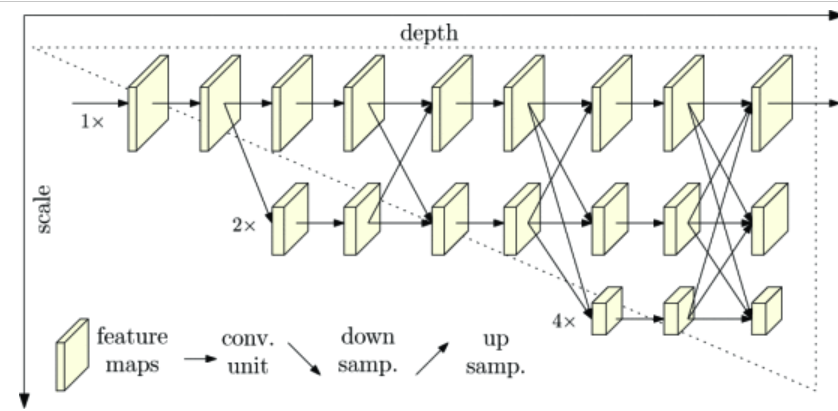
\includegraphics[width=\columnwidth]{figure1.png}
    \caption{Parallel multi-resolution subnetworks and repeated multi-scale fusion in HRNet~\cite{sun2019hrnet}.}
    \label{fig:hrnet-architecture}
\end{figure}

Sun et al.\ proposed High-Resolution Network (HRNet), which maintains
high-resolution representations throughout the network~\cite{sun2019hrnet}. As
shown in Figure~\ref{fig:hrnet-architecture}, the core of HRNet combines
parallel multi-resolution subnetworks with repeated multi-scale fusion. The
parallel subnetworks are organized into four stages. The first stage contains
only a high-resolution branch, and each subsequent stage retains the previous
branches while adding a lower-resolution branch. This design enriches
high-resolution features with stronger semantic information. Meanwhile,
multi-scale fusion exchanges information across branches of different
resolutions to generate aligned feature maps, and repeated multi-scale fusion
performs this exchange several times. Through repeated downsampling and
upsampling between branches, HRNet produces representations with both stronger
semantic content and finer spatial detail~\cite{sun2019hrnet}. Overall, HRNet improves the precise localization of body joints in 2D.

Although precise single-person localization provides an important foundation
for 2D pose estimation, directly extending single-person methods to
multi-person scenes introduces additional challenges. Cao et al.\ point out
that multi-person estimation involves uncertainty caused by the unknown number
of people in an image, spatial interference from interactions and overlap, and
rapidly increasing parsing complexity as the number of people grows
~\cite{cao2019openpose}. To address these issues, they propose Part Affinity
Fields (PAFs), which model the association between human body parts through a
set of 2D vector fields, together with confidence maps that indicate the
locations of individual body parts~\cite{cao2019openpose}. Compared with
traditional top-down methods that reuse single-person pose estimation and prior
bottom-up methods, this design enables more efficient identification and
reconstruction of unstructured pairwise relationships among body parts in
multi-person settings~\cite{cao2019openpose}.

\begin{figure}[H]
    \centering
    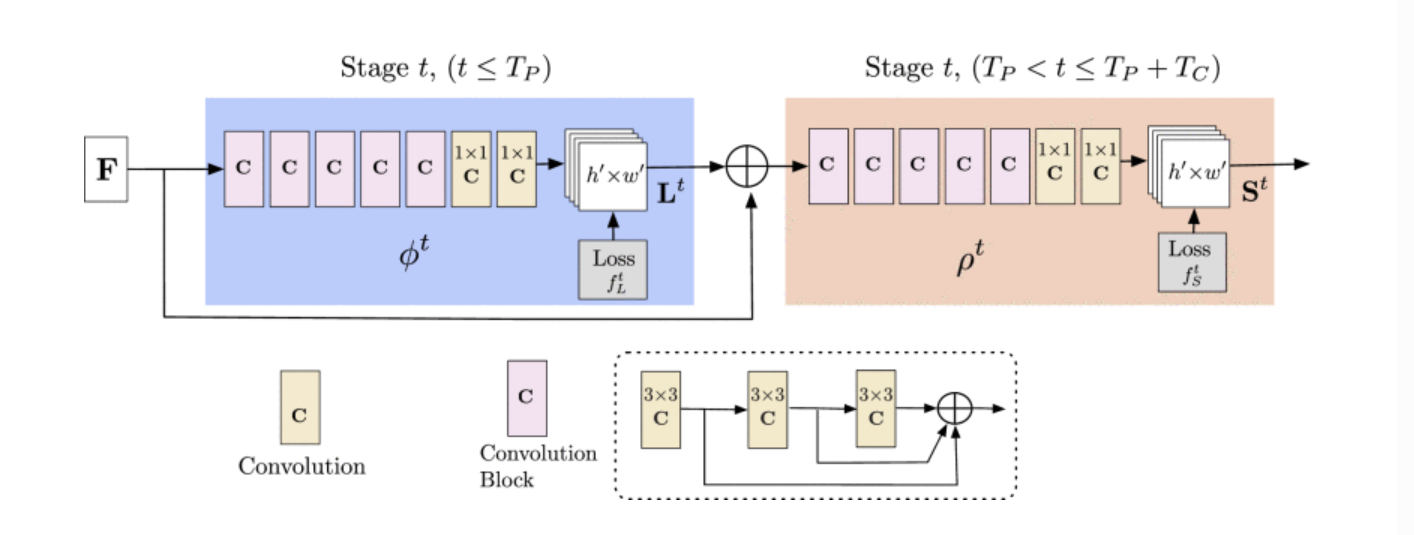
\includegraphics[width=\columnwidth]{figure2.png}
    \caption{Multi-stage prediction network used in OpenPose~\cite{cao2019openpose}.}
    \label{fig:openpose-pipeline}
\end{figure}

The OpenPose system takes a $w \times h$ color image as input and applies a
multi-stage prediction network based on Convolutional Neural Networks (CNNs),
as shown in Figure~\ref{fig:openpose-pipeline}~\cite{cao2019openpose}. The
network iteratively refines both PAFs and confidence maps. In the design, a
$7 \times 7$ convolution is replaced by three consecutive $3 \times 3$
convolutions, which reduces the operation count from $2 \times 7^2 - 1 = 97$
to $51$~\cite{cao2019openpose}. A spatially weighted loss is further used to
handle the fact that not all individuals can be fully labeled in crowded
scenes. For multi-person parsing, Cao et al.\ simplify the global matching
problem with a spanning-tree skeleton and bipartite matching over multiple
limbs, and then solve the final association through greedy inference
~\cite{cao2019openpose}. Generally, OpenPose shifts the focus from precise single-person localization to scalable multi-person association.

% -----------------------------------------------------------------------------
\section{From 2D Pose Representation to 3D Human Recovery}
The two methods discussed above produce different forms of 2D output. HRNet
represents the locations of body joints as keypoint probability heatmaps,
whereas OpenPose reconstructs posture through confidence maps, Part Affinity
Fields, and a non-fully-connected tree structure for multi-person parsing.
However, from a practical perspective, using 3D human recovery as the final
output is more meaningful, because it provides a more complete description of
human pose, body orientation, and shape.

\begin{figure}[H]
    \centering
    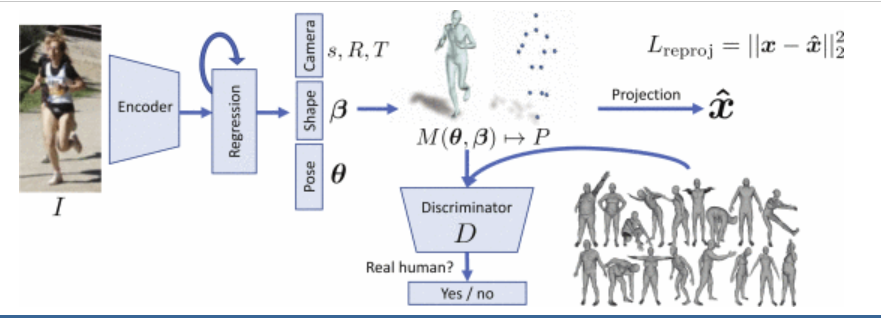
\includegraphics[width=\columnwidth]{figure3.png}
    \caption{HMR directly regresses SMPL parameters from a single RGB image to recover a 3D human mesh~\cite{kanazawa2018hmr}.}
    \label{fig:hmr-pipeline}
\end{figure}

Against this background, methods focusing on 3D joints have emerged.
Nevertheless, because such approaches still rely on mapping 2D joints to 3D
parameters, some image information is inevitably lost. Kanazawa et al.\
proposed an end-to-end method called Human Mesh Recovery (HMR), which directly
predicts 3D model parameters from image pixels~\cite{kanazawa2018hmr}. HMR
regresses the pose, shape, and camera parameters of the parameterized human
body model SMPL from a single RGB image, thereby generating a complete 3D
human mesh representation, as shown in Figure~\ref{fig:hmr-pipeline}. Its core
idea is twofold. On the one hand, a 2D reprojection loss ensures that the
predicted 3D joints, when projected back to the image plane, align with the 2D
annotations. On the other hand, an adversarial prior constrains the recovered
results to remain within reasonable distributions of human poses and body
shapes. This design addresses two major difficulties: the lack of reliable 3D
annotations in real-world scenes and the inaccuracy of 2D-to-3D conversion
caused by depth ambiguity~\cite{kanazawa2018hmr}.


% -----------------------------------------------------------------------------
\section{Connections and Limitations}
When establishing connections among the three methods, it is necessary to
revisit why Kanazawa et al.\ rejected traditional approaches that focus only
on 3D joints. HMR does not negate 2D pose estimation itself; rather, it
rejects the two-stage process that first compresses an image into sparse 2D
keypoints and then relies only on these keypoints for 3D reconstruction
~\cite{kanazawa2018hmr}. Once image information is simplified to a small number
of 2D joint positions, substantial cues about body contour, orientation, local
occlusion, and shape detail are lost~\cite{kanazawa2018hmr}. In contrast,
although HRNet and OpenPose still output 2D representations, they improve the
accuracy of single-person keypoint localization~\cite{sun2019hrnet} and
body-part association in multi-person scenes~\cite{cao2019openpose},
respectively, thereby providing stronger 2D structural evidence for subsequent
3D reconstruction. In this sense, the three methods are not mutually
exclusive, but can instead form a progressive technical pathway from 2D pose
analysis to 3D human recovery.

In addition, each method has its own limitations:
\begin{itemize}
    \item HRNet: Because it maintains high-resolution representations throughout
    the network, its computational cost is relatively high.
    \item OpenPose: Its output remains sensitive to complex occlusion and
    crowded scenes. When a person is too small or lacks detail, the prediction
    may deviate substantially.
    \item HMR: Its output is still affected by ambiguity, model assumptions,
    and supervision constraints.
\end{itemize}


% -----------------------------------------------------------------------------
\section{Future Directions and Conclusion}
From HRNet to OpenPose, and then to HMR, these methods demonstrate the
possibilities of human pose estimation in computer vision, from more accurate
single-person 2D pose representation to complex multi-person 2D pose
estimation and further toward complete 3D human body recovery. Together, these
three methods indicate that progress in human pose estimation depends not only
on more complex network architectures, but also on richer representations and
more effective supervision strategies. At the same time, they expose several
remaining limitations, which motivate future research directions. For example,
performing 3D human body recovery in multi-person scenarios remains
challenging, especially in the presence of complex spatial interactions and
occlusion, and achieving stable and accurate 3D recovery in such settings
still requires further exploration.


\nocite{cao2019openpose,sun2019hrnet,kanazawa2018hmr}

{\footnotesize
\bibliographystyle{IEEEtran}
\bibliography{refs}
}

\end{document}
